
 
 %Research projects should always be based on previous research on the same and/or related topics. This should be described as a background to the thesis with adequate bibliographical references. If the material needed is too voluminous to fit nicely in the review part of the introduction, it can be presented in a separate background chapter.
In order to get a theoretical overview of topics related to the subject of my thesis, the concept of \acrfull{sg} is explained, as well as aspects related to the \acrshort{sg} architecture, and \acrshort{sg} vulnerabilities.\\  

However, before studying the \acrshort{sg} in more detail,  some introductory terms are covered.  



\section{Critical (Information) Infrastructure}

The term Critical Infrastructure, denotes infrastructure critical to the operation of some function, or service, vital to its recipients. As a result of the society being more dependant on the availability of electronic services, the flow of electricity from the \acrshort{pg} \acrfull{ci} is dependant on networking provided by \acrfull{cii}.
\textbf{\acrfull{ci}} is, in  \cite{luiijf2012understanding}, defined as ... 
 \begin{quote}
"... an asset, system or part thereof located in a
nation which is essential for the maintenance of vital societal functions, health, safety,
security, economic or social well-being of people, and the disruption or destruction of
which would have a significant impact in that nation as a result of the failure to maintain
those functions." \cite[p. 53]{luiijf2012understanding}     
 \end{quote}
 

\textbf{\acrfull{cii}} is, in  \cite{luiijf2012understanding}, defined as ...
 \begin{quote}
" ... those interconnected information
systems and networks, the disruption or destruction of which would have a
serious impact on the health, safety, security, or economic well-being of citizens, or
on the effective functioning of government or the economy." \cite[p. 53]{luiijf2012understanding}     
 \end{quote}


The \acrshort{cii} is fundamental to the proper operation of the \acrshort{ci}, and is dependant on the availaibility of \acrfull{ict} and \acrfull{telco} \acrlong{ci}, as 
indicated by figure \ref{fig:CI-CIII}


\begin{figure}[ht]
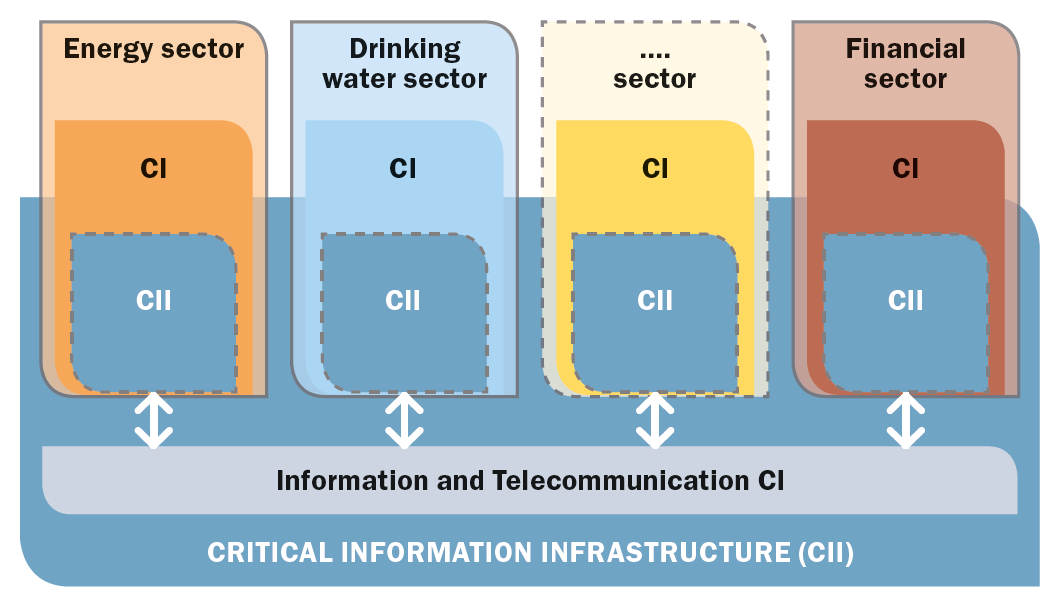
\includegraphics[width=\linewidth]{figures/CI-CII.png}
\caption[CI/CIII in the ICT and TELCO sectors]{Sector CI and CII dependency on ICT and TELCO CI. \cite{luiijf2016gfce}}
\label{fig:CI-CIII}
\end{figure}


\subsection{Critical (Information) Infrastructure Protection}

As presented in figure \ref{fig:CI-CIII}, \acrfull{ci} depends on \acrfull{cii}, as \acrshort{cii} is required in order for a distributed \acrshort{ci} like the \acrshort{sg} to operate as required. Figure \ref{fig:CI-CIII-Security} shows the relationship between Critical Infrastructure Protection and Critical Information Infrastructure Protection, as the cyber security strategies related to \acrshort{ci} protection.


\begin{figure}[ht]
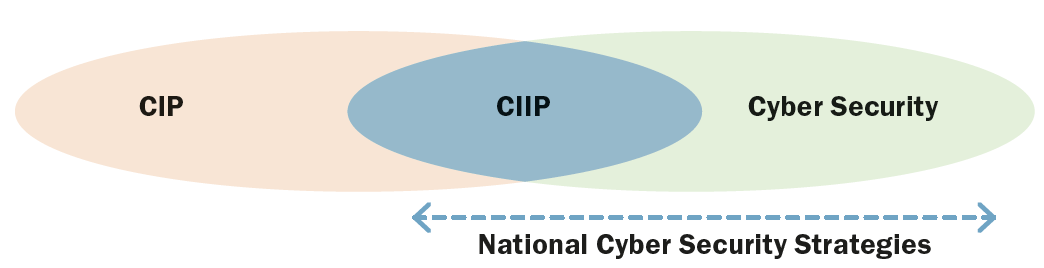
\includegraphics[width=\linewidth]{figures/CIP-CIIP-Security.png}
\caption[CIP-CIIP relations]{Relationship between Critical Infrastructure Protection and Critical Information Infrastructure Protection. \cite{luiijf2016gfce}}
\label{fig:CI-CIII-Security}
\end{figure}












\section{Cyber-Physical System}

As described by \citeauthor{humayed2017cyber} in \cite{humayed2017cyber}, a \acrfull{cps} is characterised by using a computer-based system in order to control and monitor systems of the physical world. The \acrshort{cps} is utilised in order to control physical systems from various fields of applications. Humayed et. al., in \cite{humayed2017cyber}, describes as various appliances as \acrfull{ics}, Medical Devices, and \acrlong{sg}.
The Smart Grid, therefore, is an example of a \acrfull{cps}, consisting of the physical system of a Power Grid, under the control of a network/Cyberspace-connected system. 
The \acrshort{sg} is, as described by several papers, like \cite{humayed2017cyber}% \#NEWREF and \cite{alcaraz2012security}
, under the control of a \acrfull{scada} system.




\










\subsection{Smart Grid as Critical Infrastructure}



As described in \cite{colesniuc2013cyberspace}, information technology is critical to the successful operation of the modern society.




 
 The EU Commission defines, in \cite{eu2008council}, \textit{National Critical Infrastructure}, to mean...:
 
 \begin{quote}
    "... an asset, system or part thereof
located in Member States which is essential for the maintenance of vital societal functions, health, safety, security,
economic or social well-being of people, and the disruption
or destruction of which would have a significant impact in a
Member State as a result of the failure to maintain those
functions"   \cite[p.  L 345/77]{eu2008council}  
 \end{quote}
 
 The disruption of an \textit{European Critical infrastructure}, according to  \cite{eu2008council}... \\ "...would have a significant impact of at least Two member states."

Recognised as critical infrastructure, the availability of the \acrlong{sg} is of paramount importance to the society. 



\subsection{Time Synchronisation Sources}

As described by \citeauthor{moussa2016security} in \cite{moussa2016security}, both PTP and GNSS is able to achieve the precision level required, as opposed to NTP and PPS.  Based on this observation, the \acrshort{tsa} Detection and Mitigation coverage is limited to \acrshort{gnss} and  \acrshort{ptp} systems only.




\subsubsection{Global Navigation Satellite Systems}

A \acrfull{gnss}, is a system of communication satellites orbiting the Earth, in order to determine the current position for, usually,\footnote{\acrlong{sg} systems utilises \acrshort{gnss} systems for time synchronisation, not navigational, purposes.} navigation  purposes. As described by \citeauthor{schmidt2016survey} in \cite{schmidt2016survey}, there exists several \acrshort{gnss} constellations,\footnote{In \cite{schmidt2016survey}, both the United States "GPS" and the Russian "GLONASS" systems, as well as the European "Galileo" and the Chinese "Beidou-2" systems are mentioned.} each being classified as "strikingly similar" to the other \acrshort{gnss} systems. 



%Therefore, any description of \acrshort{gnss} systems, as well as attacks targeting them, will be considering the well-known \acrfull{gps} system only.





As described by \citeauthor{schmidt2016survey} in  \cite{schmidt2016survey},  a \acrshort{gnss} system transmits three different messages:

\begin{enumerate}
    \item A PVT ranging signal for Position, Velocity, and Timing.
    \item Precise Ephemeris\footnote{Ephemeris is calculated based on prior observations of astronomical object trajectories} data, is specifying the exact location of each satellite.
    \item An almanac used in order to select satellites for tracking, based on the known location of all satellites. 
    
\end{enumerate}

$$r(t)=\sum_{k=1}^{32}H_{k}(2P_{c})^{\frac{1}{2}}(C_{k}(t)\oplus D_{k}(t))\cos{2\pi}(f_{L1}+\Delta f_{k})t+n(t) $$


As further described by \citeauthor{schmidt2016survey}, satellites from any other \acrshort{gnss} constellation may be used in order to avoid problems related to poor reception or blackout which would, possibly be the result of using same constellation satellites only.


The \acrshort{gnss} signal is utilised in order to provide time synchronisation between \acrshort{sg} \acrshort{pmu} devices, in order to enable the \acrshort{wams} system operators to get the best available 
view of \acrshort{sg} distribution system state.


\subsubsection{Description of GSSN time synchronisation}
The time signal available from \acrfull{gnss} systems is by several papers described as the major contributor to the wide-spread usage of \acrshort{pmu}s in order to monitor \acrlong{sg} energy flow status. 







The GPS signal transmits timing information, which enables 


$$t_{UTC}=t_{rcv}-t_{p}-\Delta t_{UTC}$$
A synchrophasor is, as described by 



%\textbf{TO DO:}
%\textit{Introduction:}

%\textit{What is it?}
%\textit{Which functions does it have?}





%Explain TimeSync 








A periodic signal $x(t)=X_m\cos\left(\omega t+\phi \right)$ has, according to \Cite{schofield2018design}, a synchrophasor representation $\mathbf{X}$, defined by $ \mathbf{X} = \frac{X_m}{\sqrt{2}}e^{j\phi} $ where $ \mathbf{X} = |X| = X_m / \sqrt{2} $ is  the RMS and $  \phi = angle(\mathbf{X}) $ is the angle.


%\[x(t)=X_m\cdot\cos\left(\phi + \int\displaylimits_{-\infty}^t\omega (\tau)\cdot\mathrm{d}\tau\right)\]

%\[\overline{X} = X_m{\angle\phi} \]








\section{cyber attacks}
\subsection{Introduction}
\subsection{type of attacks}
\subsection{Threat Actors}
\subsubsection{Introduction}
\subsubsection{Type of Threat Actors}
\subsection{Attack strategies}
